\section{Learning Theory}

\subsection{No Free Lunch Theorem}

Assuming that the training set \(\mathcal{D}\) can be learned correctly by all algorithms, averaged over all target functions no learning algorithm gives an off-training set error superior to any other:

\[\sum_F [\mathbb{E}_1 (E \mid F, \mathcal{D}) - \mathbb{E}_2(E \mid F, \mathcal{D})] = 0\]

where \(F\) is the set of all possible target functions, \(E\) is the off-training set error, and \(\mathbb{E}_1, \mathbb{E}_2\) are expectations for two learning algorithms.

\subsection{A Conservation Theorem of Generalisation Performance}

For every possible learning algorithm for binary classification the sum of performance overall possible target functions is exactly zero! \\

On some problems we get positive performance, so there must be other problems for which we get an equal and opposite amount of negative performance.

\subsection{PAC Learning}

There is a whole section on this... Something about Boosting

\subsection{Vapnik-Chervonenkis (VC) Dimension}

There is also a section on this... Something about SVM

\subsection{Mistake Bounds}

How many mistakes before convergence? \\

\subsubsection{\texttt{WINNOW}}

\begin{itemize}
    \item \texttt{WINNOW} is an online, mistaken-drive algorithm. Similar to perceptron but converges faster.
    \item Designed to learn in the presence of many irrelevant attributes. Key improvement: number of mistakes grows only logarithmically with number of irrelevant attributes.
    \item Key idea: use a multiplicative weight update scheme (as in Boosting).
\end{itemize}

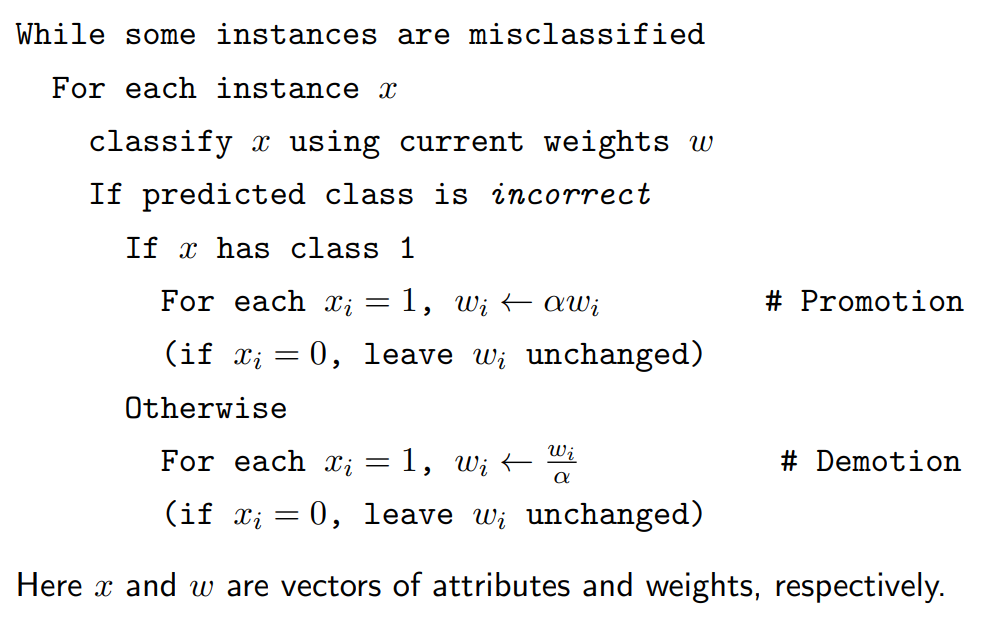
\includegraphics[scale=0.6]{assets/winnow.png}

\subsection{The \texttt{WEIGHTED MAJORITY} Algorithm}

\begin{itemize}
    \item learn to predict by weighted vote of set of prediction algorithms
    \item learns by updating weights for prediction algorithms
    \item any prediction algorithm simply predicts value of target concept given an instance; a prediction algorithm can be elements of hypothesis space \(H\) or even different learning algorithms
    \item if there is inconsistency between prediction algorithm and training example then reduce weight of prediction algorithm
    \item bound number of mistakes of ensemble by number of mistakes made by best prediction algorithm
\end{itemize}

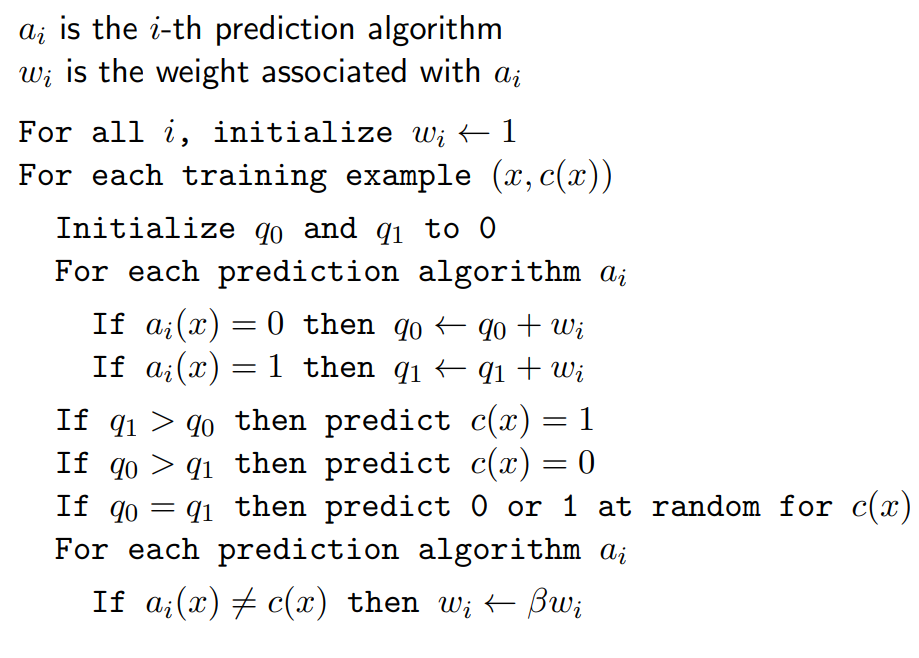
\includegraphics[scale=0.6]{assets/weighted_majority.png}
